\section{\acl{HMM}}
\label{mainsec:hmm}
\textit{Paul Pasler, Sebastian Rieder}

Das \acl{HMM} ist ein stochastisches Modell für sequentielle Daten und wird vor allem in der Spracherkennung und in der Bioinformatik eingesetzt.

In den folgenden beiden Abschnitten werden die Entstehung und Konzepte der \acl{MK} und des \acl{HMM} aufgezeigt.
Abschnitt \ref{sec:preproc} befasst sich mit der Aufbereitung der Daten für das Training und die Klassifizierung der Gesten.
Die Implementierung und Anwendung des \acl{HMM} werden im Abschnitt \ref{sec:impl} näher erläutert. Im letzten Abschnitt werden die Ergebnisse 
evaluiert und ein Fazit mit Ausblick gezogen.  
 
  %%%%%%%%%%%%%%%%%%
  %  MARKOV-KETTE  % 
  %%%%%%%%%%%%%%%%%%  
\subsection{\acl{MK}} \label{sec:chain}
Grundlage des \acl{HMM} war die vom russischen Mathematiker Andrej Andrejewitsch Markov 
(1856 - 1922, siehe \cite{markov1913}) entwickelte \acl{MK}. Zu Beginn des
20. Jahrhunderts beschäftigte er sich als erster mit einer statistischen Beschreibung von Zustands- und Symbolfolgen. 
Er führte eine statistische Analyse der Buchstabenfolge des Textes ``Eugen Onegin'' von Alexander 
Pushkin.

Eine \acl{MK} beschreibt einen zeit-diskreten Prozess \((X_t)_{t\in\mathbb{N}_0}\) mit einem abzählbaren Zustandsraum \(S\) \cite{stochMod}.
Da die Verteilung der Zufallsvariable \( S(t)\) nur von den vergangenen Zuständen abhängt gilt sie als kausal. \cite[48]{mmmFink}
Für eine Markov-Kette 1. Ordnung gilt die Markov Eigenschaft, dann wird sie auch als ``einfach'' bezeichnet: \\
\( \forall t \in \mathbb{N} : P (X_{t+1} = s_{t+1} | X_0 = s_0, \ldots , X_{t-1} = s_{t-1}, X_{t} = s_{t}) = P ( X_{t+1} = s_{t+1} | X_{t} = s_{t} ) \) \\
Dies beschreibt die Gedächtnislosigkeit des Prozesses und bedeutet, dass der nächste Zustand nur vom direkten Vorgänger abhängt.
Weiterhin wird eine \acl{MK} als stationär bezeichnet, wenn alle Wahrscheinlichkeiten unabhängig von der Zeit sind.

Als Übergangswahrscheinlichkeit bezeichnte man die bedingte Wahrscheinlichkeit \(P ( X_{t+1} = s_{t+1} | X_{t} = s_{t} ) \), dass auf 
\( s_{n}\) der Nachfolgezustand \( s_{n+1}\) folgt. Diese Wahrscheinlichkeiten werden üblicherweise zu einer Übergangsmatrix zusammengefasst: \\
\( A = [a_{ij}] = [ P (X_t = j) | P (X_{t-1} = i) ] \)
\( \forall i, j \in S, \sum_{j \in S} p_{ij} = 1 \) \\
Weiterhin benötigt der Prozess einen Vektor für den Anfangzustand \( t = 0 \):
\( \Pi = [ \pi_i] = [ P (X_0 = i) ] , i \in S \)

So lässt sich eine Markov-Kette durch Zustandsraum \(S\), den Übergangsmatrix \( A \) und einen Anfangszustand \( \Pi \) definieren.
Veranschaulichen lässt sich eine Markov Kette als gerichtetes Zustandsdiagramm (Abb. \ref{fig:simple_mc})
\begin{figure}[htbp] \centering
    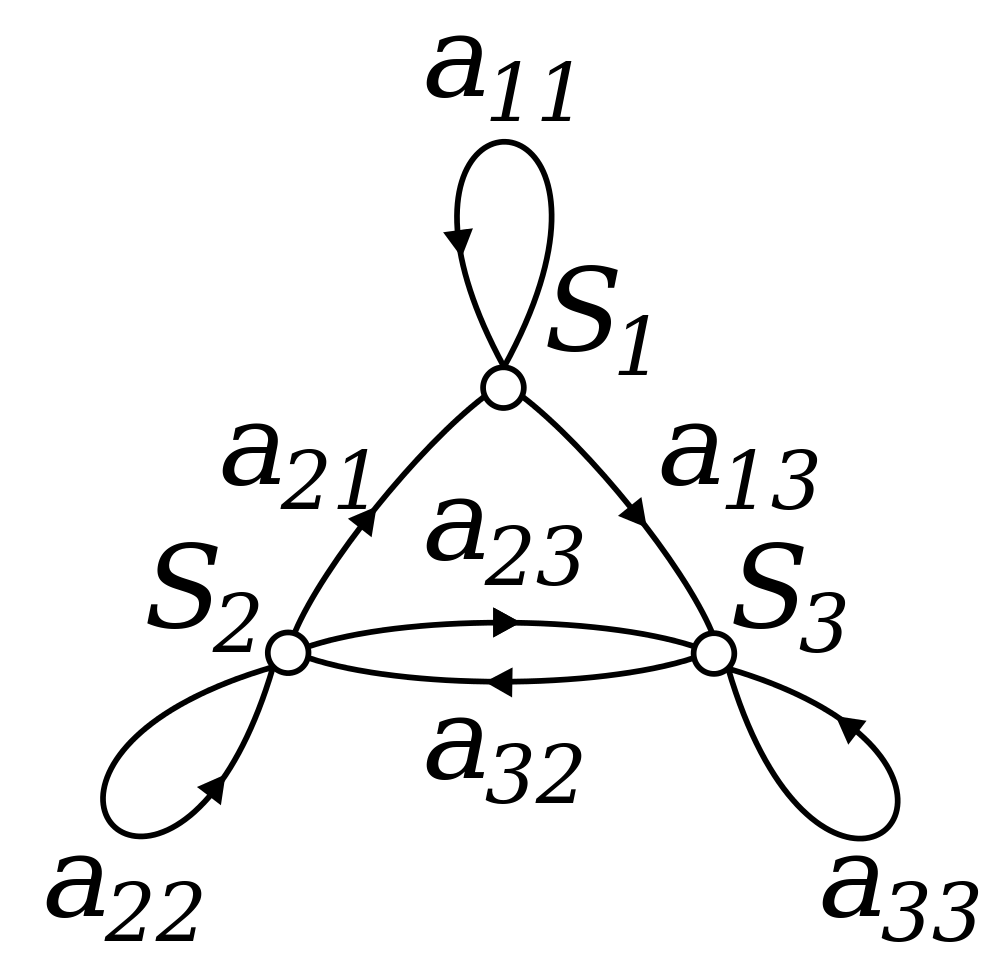
\includegraphics[width=0.33\textwidth]{markov/simple_mc.png}
    \caption{Einfaches Zustandsdiagramm einer \acl{MK} (de.wikipedia.org/wiki/Markow-Kette)}
    \label{fig:simple_mc}
\end{figure}



Eine \acl{MK} ist eine Sequenz von Zufallsvariablen \( X_1, x_2, X_3, \ldots\) und beschreibt einen speziellen stochastischen Prozess, 
der aufgrund der Vorgeschichte, Aussagen über die Zukunft machen kann. 
Eine \acl{MK} kann als Gerichteter Graph mit Zuständen \(S\) und mit Übergangswahrscheinlichkeiten \(X_i\) an den Kanten beschrieben werden. 

Sie ist definiert durch eine endlich Menge an Zuständen \( S = \{ s | 1 <= s <= N \} \) und der diskreten Zeit \( t = 0, 1, 2, \ldots \) \\


  %%%%%%%%%%%%%%%%%%
  %  HIDDEN-MARKOV  % 
  %%%%%%%%%%%%%%%%%%
\subsection{\acl{HMM} und \acl{GMM}}  \label{sec:hmm}
Der amerikanischen Mathematiker Leonard E. Baum (* 1931) und andere Autoren entwickelten auf Basis der \acl{MK} Ende der 
sechziger Jahre das \acl{HMM}. Erste \acl{HMM}-Applikationen wurden zur Spracherkennung und später auch in der Bioinformatik 
zur Analyse von Nukleotid- und Proteinsequenzen eingesetzt. 

Ein \acl{HMM} erweitert eine \acl{MK} um eine weiteren Zufallsprozess und ist somit ein zweistufiger stochastischer Prozess \cite[67]{mmmFink}
zustandsspezifische Ausgabe und eine statistisch modellierte Zustandsfolge. 


Es wird beschrieben durch:\\ 
\( \lambda = (S;V;A;B;\pi)\)
\begin{itemize}
     \item Endlich Menge von Zuständen \\
           \( S = \{ s | 1 <= s <= N \} \)
     \item Alphabeth der Emissionen \\
           \( V = \{ v | 1 <= v <= M \} \)
     \item Matrix der Zustandsübergangswahrscheinlichkeiten \\
           \( A = \{ a_{ij} | a_{ij} = P(S_t = j | S_{t-1} = i) \} \)
     \item Matrix der Emissionswahrscheinlichkeiten \\
           \( B = \{ b_{jk} | b_{jk} = P(O_t = o_k | S_t = j) \} \)
     \item Vektor von Zustandsstartwahrscheinlichkeiten \\
           \( \pi = \{ \pi_i | \pi_i = P(S_1 = i) \} \) 
\end{itemize}

Das Konzept des \acl{HMM} kann laut \cite{rabiner} in drei Problemstellungen eingeteilt werden:
\begin{itemize}
  \item Evaluierungsproblem: 
  \item Dekodierungsprobem: Finde interne Abläufe für eine gegebene Observationsfolge
  \item Trainingsproblem: Finde Modellparameter für gegebene Besispieldaten
\end{itemize}




Um das Training und die Klassifizierung möglichst genau und perfomant umzusetzen, 
ist es notwendig die aufgenommenen Daten auzubereiten, dies ist Thema des nächsten Abschnitts


  %%%%%%%%%%%%%%%%%%%
  %  PREPROCESSING  % 
  %%%%%%%%%%%%%%%%%%%
\subsection{Datenaufbereitung} \label{sec:preproc}
Eine Aufnahme wird beschrieben durch ein zwei-dimensionales Array aus 32 Frames mit jeweils 64 Frequenzwerten.
Im Ruhezustand bildet sich ein Signalpeak um die ausgesendete Frequenz (18.500hz).
Ziel ist es die Daten zu normieren und die Datenmenge zu reduzieren, um das Trainingergebnis bzw. Performance zu verbessern.
Weiterhin wird versucht die relevanten Werte einer Geste aus der Aufnahme zu extrahieren.

Da sich Änderungen durch eine Bewegung sehr Nahe am gesendeten Signal liegen, werden die Daten im 
Frequenzbereich von 18.000hz bis 19.000hz betrachtet, die Daten vermindern sich von 64 auf 13 Werte. 
Dazu wird jede Geste auf einem Intervall von 0 bis 1 normalisiert (Geteilt durch den jeweiligen Maximalwert) und 
auf zwei Nachkommstellen gerundet. 
Alle Werte unterhalb eines Schwellwerts (0.1) werden zudem abgeschnitten, um niedrig amplitudiges Rauschen zu vermindern. 
So wird im Idealfall nur das gesendete Signal und Frequenzänderungen durch eine Geste dargestellt.

Wichtig ist nun den Beginn und das Ende einer Geste zu finden. Hierzu werden pro Frame alle Werte addiert 
und das Maximum als Mittelpunkt der Geste genutzt. Von diesem Gestenhöhepunkt werden jeweils 6 Frames davor und danach mitgenutzt.

So wird aus einem 32 x 64 Array pro Geste ein 13x13 Array.

\begin{figure}[htbp] \centering
    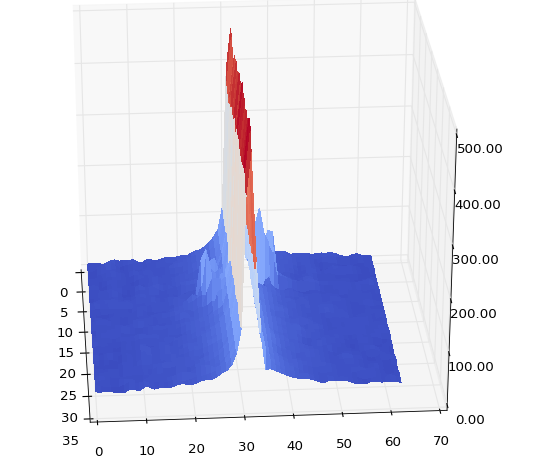
\includegraphics[width=0.4\textwidth]{markov/data_raw.png}
    \caption{Rohdaten direkt vom Recorder (\acl{RLO} Geste) mit gefundener Gestenmitte (Roter Punkt)}
    \label{fig:data_raw}
\end{figure}

\begin{figure}[htbp] \centering
    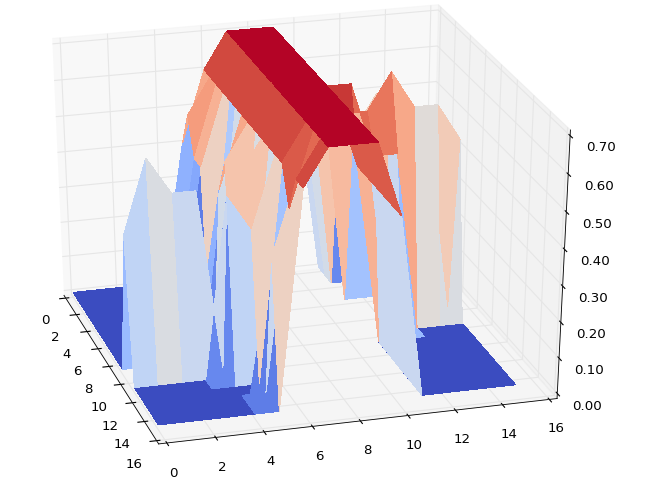
\includegraphics[width=0.4\textwidth]{markov/data_preproc.png}
    \caption{Daten nach der Vorverarbeitung (\acl{RLO} Geste)}
    \label{fig:data_preproc}
\end{figure}

\begin{figure}[htbp] \centering
    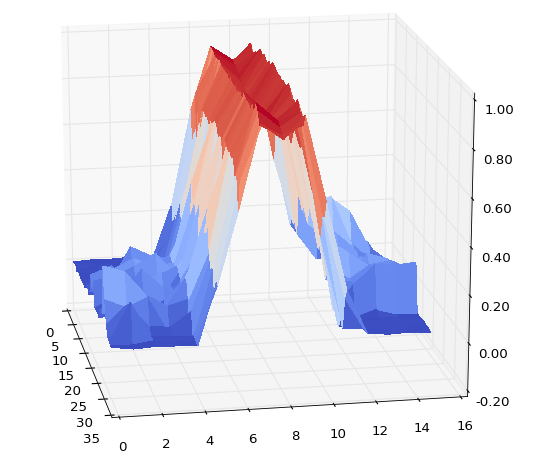
\includegraphics[width=0.4\textwidth]{markov/data_gmm.png}
    \caption{Sampledaten aus dem trainierten \acl{GMM} (\acl{RLO} Geste)}
    \label{fig:data_gmm}
\end{figure}

  %%%%%%%%%%%%%%%%%%%%%
  %  IMPLEMENTIERUNG  % 
  %%%%%%%%%%%%%%%%%%%%%
\subsection{Implementierung}  \label{sec:impl}
Wir haben uns für die scipy HMM implementierung entschieden. 
Genutzt wird ein \acl{HMM} mit \acl{GMM} entschieden.


  %%%%%%%%%%%%
  %  RESULT  % 
  %%%%%%%%%%%%
\subsection{Evaluation und Fazit}  \label{sec:result}
Das Hidden Markov Modell eignet sich grundsätzlich sehr gut für die gestellte Aufgabe. Da es mit sequenzielle Daten (Frames) umgehen 
kann und ursprünglich für die Spracherkennung entwickelt wurde. Ob nun aus einem Tonsignal (versteckte Zustände) ein Wort oder 
eine Geste (Emissionen) erkannt werden soll, ist vom Vorgehen ähnlich. Ein Vorteil ist zudem, dass die Ausführungsgeschwindigkeit
 der Geste, bei geeigneter Aufnahmelänge, die Klassifizierung nicht unbedingt beeinflusst, da dann länger im selben versteckten 
 Zustand verblieben wird.
Ein Nachteil dieser Methode ist, dass keine absoluten Klassifizierungen durchgeführt werden können. Es werden nur Wahrscheinlichkeiten für alle möglichen Klasse berechnet. So muss entschieden werden, ob die Wahrscheinlichkeit für eine Klasse hoch genug ist, sodass diese als Geste identifiziert werden kann.
